%!TEX root = ../main/main.tex
\section{Data management view} % (fold)
\label{sec:data_management}
This section focuses on policies and data storing management.\\
\subsection{Data Policy} % (fold)
\label{sub:data_policy}
\subsubsection{Automatic data elimination} % (fold)
\label{ssub:data_elimination}
Data about \emph{Users} and \emph{Taxi Drivers} is never automatically eliminated from the system.\\
However rides logs are kept for 12 months to save storage space and to speed up queries.
% subsubsection data_elimination (end)
\subsubsection{Data caching policy} % (fold)
\label{ssub:data_caching}
In order to reduce the load on the \emph{Server} and to speed up user's query response, all the data that does not change frequently (like the user's profile data) is saved locally on the device and reloaded only when a modification of the profile occurs.

% subsubsection data_caching (end)
\subsection{Data storing} % (fold)
Here is a presentation of the data base schema that will have to be employed:
\newpage
\label{sub:data_storing}
\begin{figure}[h!t]
\caption{ER Diagram}
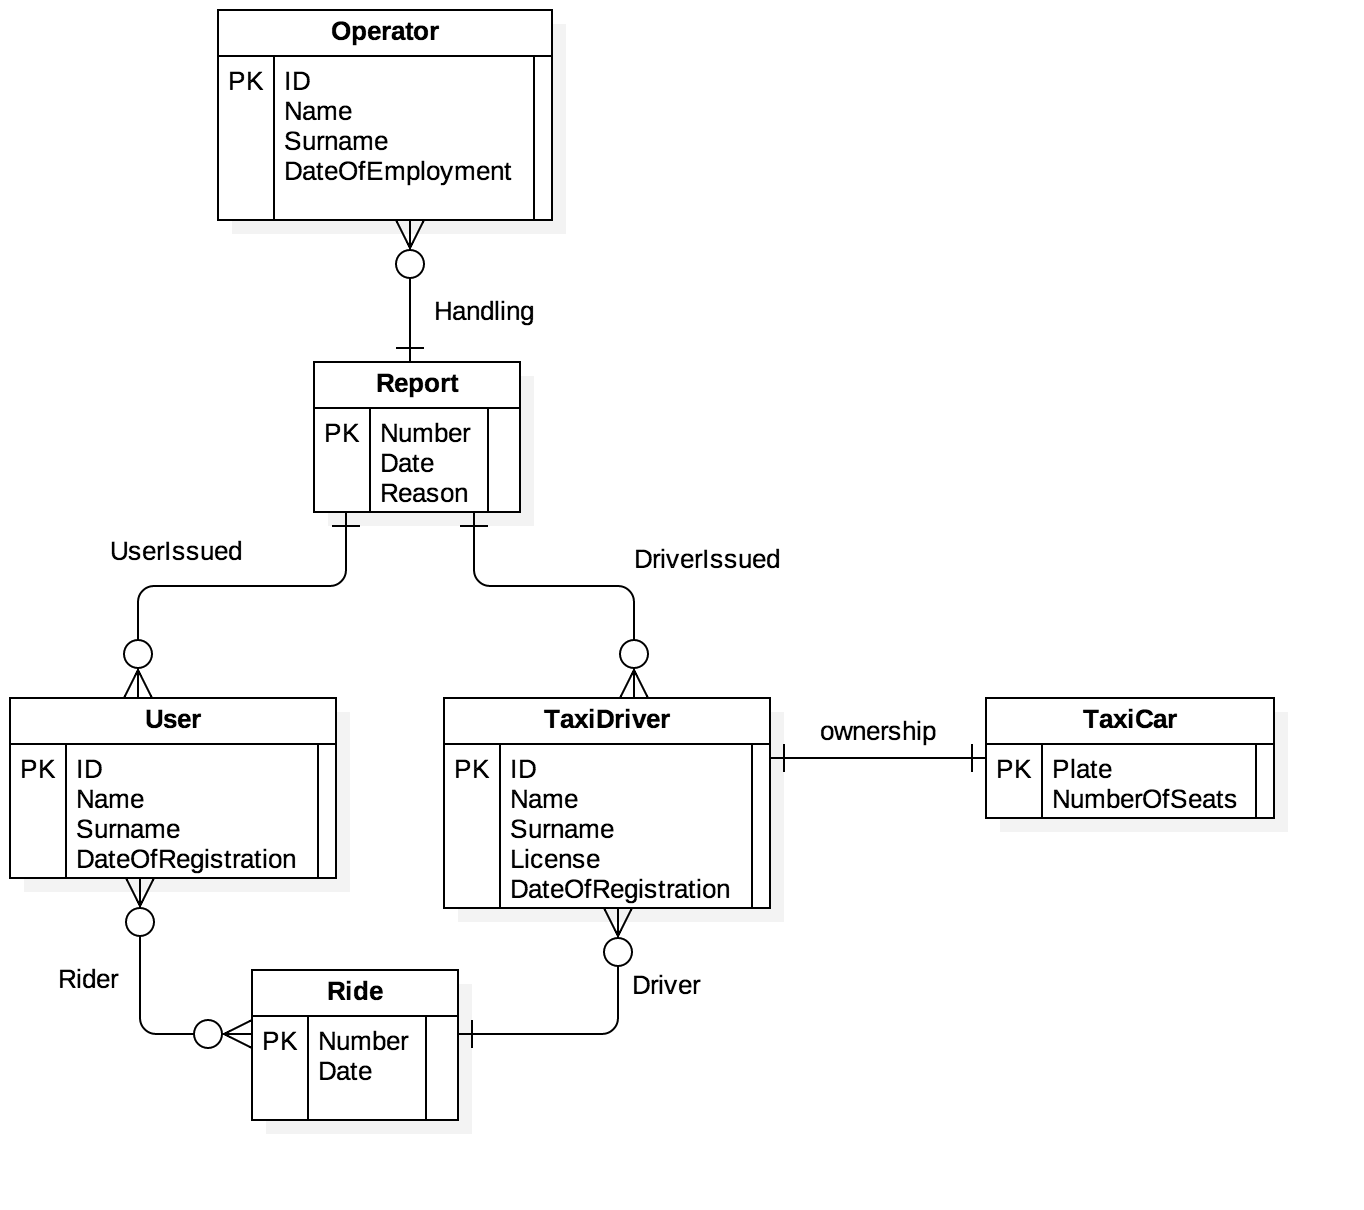
\includegraphics[width=\textwidth]{diagram/png/ERD}
\centering
\end{figure}
\newpage

\subsubsection{ER Diagram analysis} % (fold)
\label{ssub:er_diagram_analysis}

The database schema is relatively simple and slim.
Here is an explanation of all the entities and relationships:

\paragraph{Entities} % (fold)
\label{par:entities}
The schema is composed of a total of 6 entities:

\begin{itemize}
	\item {\textbf{Operator}} \\
		Its primary key is a unique ID, and it is the number of his/her identity card.
		Some of his/her personal information is stored, together with the date in wich he/she was employed.
	\item {\textbf{User}} \\
		Its primary key is a unique ID, and it is the number of his/her identity card.
		Some of his/her personal information is stored, together with the date in wich he/she registered to the service.
	\item {\textbf{TaxiDriver}} \\
		Its primary key is a unique ID, and it is the number of his/her identity card.
		Some of his/her personal information is stored, together with the date in wich he/she registered to the service.
		The taxi license is also stored for this entity.
	\item {\textbf{TaxiCar}} \\
		Its primary key is the license plate. Each \emph{TaxiCar} has also the number of passenger seats available.
	\item {\textbf{Ride}} \\
		Its primary key is a unique number. In this entity it is also stored the date in which the ride has happened.
	\item {\textbf{Report}} \\
		Its primary key is a unique number. The other attributes are the date of the report and the reason of the report.
\end{itemize}


% paragraph entities (end)
\newpage
\paragraph{Relationships} % (fold)
\label{par:relations}
\begin{itemize}
	\item {\textbf{Handling}} \\
		This is the relation that associates each report with an \emph{Operator}, that is the one that took care of that specific \emph{Report}.\\Cardinality: 
		\begin{itemize}
			\item {\textbf{Operator side}}: 0..* \\
				This is because an \emph{Operator} may have never handled any report, or he/she may have handled multiple reports.
			\item {\textbf{Report side}}: 1 \\
				This is because a report can be handled by one and only one \emph{Operator}.
		\end{itemize}
	\item {\textbf{Issued}} \\
		There are two kinds of this relation: the \emph{User} one and the \emph{TaxiDriver} one.
		This is to keep track of which one of the two kinds of customers issued the report.
		\paragraph{UserIssued} % (fold)
		\label{par:userissued}
		This is the relation that associates the reports with a \emph{User}, that is the one that issued that specific report.\\Cardinality: 
			\begin{itemize}
				\item {\textbf{User side}}: 0..* \\
					This is because a \emph{User} may have never issued any report, or he/she may have issued multiple reports.
				\item {\textbf{Report side}}: 1 \\
					This is because a report can be issued by one and only one \emph{Person}.
			\end{itemize}
		% paragraph userissued (end)

		\paragraph{DriverIssued} % (fold)
		\label{par:driverissued}
		This is the relation that associates the reports with a \emph{TaxiDriver}, that is the one that issued that specific report.\\Cardinality: 
			\begin{itemize}
				\item {\textbf{Driver side}}: 0..* \\
					This is because a \emph{Taxi Driver} may have never issued any report, or he/she may have issued multiple reports.
				\item {\textbf{Report side}}: 1 \\
					This is because a report can be issued by one and only one \emph{Person}.
			\end{itemize}
		% paragraph driverissued (end)

	\item {\textbf{Rider}} \\
		This is the relation that associates each ride with a \emph{User}.\\Cardinality: 
		\begin{itemize}
			\item {\textbf{User side}}: 0..* \\
				This is due to the fact that a user may have never taken part to a \emph{Ride} since he has registered to the service.
			\item {\textbf{Ride side}}: 1..* \\
				This is because a \emph{Ride} must have at least one user but may have more than one if it is a \emph{Shared Ride}.
		\end{itemize}

	\item {\textbf{Driver}} \\
		This is the relation that associates each ride with a \emph{TaxiDriver}.\\Cardinality: 
		\begin{itemize}
			\item {\textbf{Driver side}}: 0..* \\
				This is due to the fact that a driver may have never taken part to a \emph{Ride} since he has registered to the service.
			\item {\textbf{Ride side}}: 1 \\
				This is because a \emph{Ride} must have exactly one and only one driver, no matter what kind of ride.
		\end{itemize}

	\item {\textbf{Ownership}} \\
		This is the relation that associates each \emph{TaxiDriver} with a \emph{TaxiCar} and vice-versa.\\Cardinality: 
		\begin{itemize}
			\item {\textbf{Driver side}}: 1 \\
				This is due to the fact that a driver must have exactly one and only one car in order to register to the service. 
			\item {\textbf{Car side}}: 1 \\
				This is because a car must have exactly one and only one driver in order to exist in the system.
		\end{itemize}
\end{itemize}

% paragraph relations (end)

% subsubsection er_diagram_analysis (end)
% subsection data_storing (end)
